% Generated by `python paper/make_figures.py`; do not edit. Every value: paper/evidence_ledger_figures.md.
\begin{figure}[t]\centering
\ifdefined\includegraphics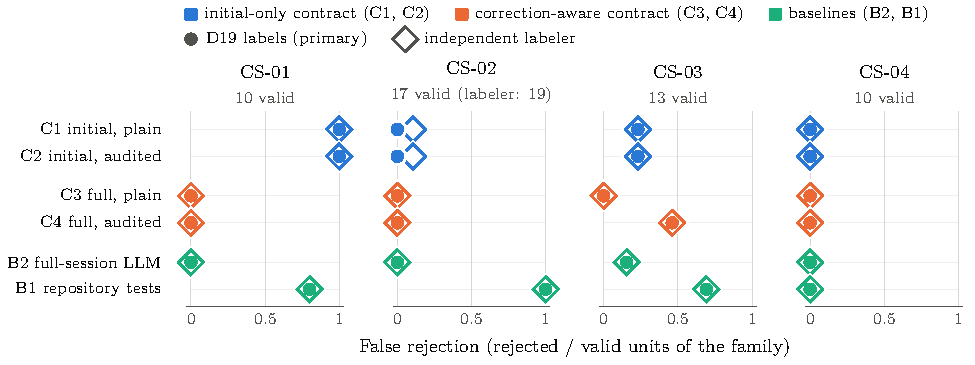
\includegraphics[width=\linewidth]{generated/figures/fresh_fr_by_family.pdf}%
\else\unfilled{figure fresh\_fr\_by\_family: main.tex must load graphicx}\fi
\caption{False rejection per family on the fresh-agent stratum (run \texttt{fresh-v1}, an automated study), the per-family display of protocol \S15.7: for each condition, the share of a family's valid units that it rejects, under D19 (filled circles) and under the independent labeler, a second labeling (open diamonds; a circle inside a diamond: both labelings give the same value). Each distinct graded patch counts once (79 units); under each family: its valid units under D19, and under the labeler where that differs. \textbf{All labels are model proposals; no human labels exist.} Four controlled families: descriptive, not inferential. In CS-02 the 2 invalid units under D19 violate only the regression norm; the labeler, which has no regression part, labels both valid. C1 and C2 do not pass CS-01's reference solution. Colour: the contract source; counts: Table~\ref{tab:fresh-family}.}\label{fig:fresh-fr}
\end{figure}
